%% !TEX root = manual.tex

\section{Discrete Event Simulation}
\label{sec:tutorial:des}
Although not necessary for using the simulator, a basic understanding of discrete event simulation can be helpful in giving users an intuition for network models and parameters.
Here we walk through a basic program that executes a single send/recv pair.
\sstmacro simulates many parallel processes, but itself runs as a single process with only one address space (\sstmacro can actually run in parallel mode, but we ignore that complication here).
\sstmacro manages each parallel process as a user-space thread (application thread), allocating a thread stack and frame of execution.
User-space threading is necessary for large simulations since otherwise the kernel would be overwhelmed scheduling thousands of threads.

\sstmacro is driven by a simulation thread which manages the user-space thread scheduling (Figure \ref{fig:des}).
In the most common (and simplest) use case, all user-space threads are serialized, running one at a time.
The main simulation thread must manage all synchronizations, yielding execution to process threads at the appropriate times.
The main simulation thread is usually abbreviated as the DES (discrete event simulation) thread.
The simulation progresses by scheduling future events.  
For example, if a message is estimated to take 5 $\mu$s to arrive,
the simulator will schedule a MESSAGE ARRIVED event 5 $\mu$s ahead of the current time stamp.
Every simulation starts by scheduling the same set of events: launch process 0, launch process 1, etc.

\begin{figure}[h!]
\centering
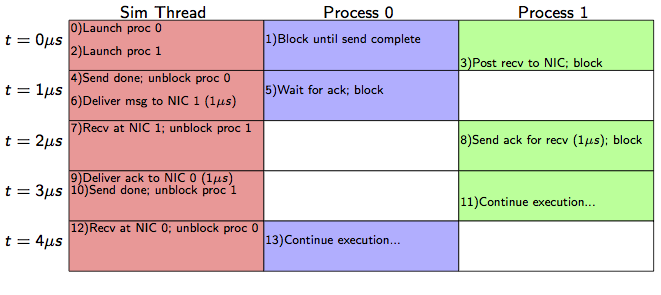
\includegraphics[width=0.95\textwidth]{figures/tikz/des/events.png}
\caption{Progression of Discrete Event Simulation for Simple Send/Recv Example}
\label{fig:des}
\end{figure}

The simulation begins at time $t=0\mu s$.  
The simulation thread runs the first event, launching process 0.
The context of process 0 is switched in, and \sstmacro proceeds running code as if it were actually process 0.
Process 0 starts a blocking send in Event 1.
For process 0 to perform a send in the simulator, it must \emph{schedule} the necessary events to simulate the send.
Most users of \sstmacro will never need to explicitly schedule events.
Discrete event details are always hidden by the API and executed inside library functions.
In this simple case, the simulator estimates the blocking send will take 1 $\mu$s.
It therefore schedules a SEND DONE (Event 4) 1 $\mu$s into the future before blocking.
When process 0 blocks, it yields execution back to the main simulation.

At this point, no time has yet progressed in the simulator.
The DES thread runs the next event, launching process 1, which executes a blocking receive (Event 3).
Unlike the blocking send case, the blocking receive does not schedule any events.
It cannot know when the message will arrive and therefore blocks without scheduling a RECV DONE event.
Process 1 just registers the receive and yields back to the DES thread.

At this point, the simulator has no events left at t=0 $\mu$s and so it must progress its time stamp.
The next event (Event 4) is SEND DONE at t=1 $\mu$s. The event does two things.
First, now that the message has been injected into the network, the simulator estimates when it will arrive at the NIC of process 1.
In this case, it estimates 1 $\mu$s and therefore schedules a MESSAGE ARRIVED event in the future at t=2 $\mu$s (Event 7).
Second, the DES thread unblocks process 0, resuming execution of its thread context.
Process 0 now posts a blocking receive, waiting for process 1 to acknowledge receipt of its message.

The simulator is now out of events at t=1 $\mu$s and therefore progresses its time stamp to t=2 $\mu$s.
The message arrives (Event 7), allowing process 1 to complete its receive and unblock.
The DES thread yields execution back to process 1, which now executes a blocking send to ack receipt of the message.
It therefore schedules a SEND DONE event 1 $\mu$s in the future (Event 10) and blocks, yielding back to the DES thread.
This flow of events continues until all the application threads have terminated.
The DES thread will run out of events, bringing the simulation to an end. 


